\documentclass[beamer]{standalone}

\begin{document}

\begin{frame}\frametitle{У чому різниця між АММ та біржами на ордер буках?}
  \begin{block}{Order Book}
    Ордер Буки (з англ. \textit{order book}) --- це список заявок на купівлю та
    продаж активу, що відображається у вигляді таблиці з ціною та об'ємом.
  \end{block}
  \begin{columns}
    \column{0.5\textwidth}
    \begin{table}
      \begin{tabular}{ c | c }
        Об'єм & Ціна \\
        \hline \hline
        1 & 10,0 \\
        \rowcolor{green} 2 & 9,95 \\
        3 & 9,87 \\
        4 & 9,71
      \end{tabular}
      \caption{Таблиця на купівлю}
    \end{table}
    \column{0.5\textwidth}
    \begin{table}
      \begin{tabular}{ c | c }
        Ціна & Об'єм \\
        \hline \hline
        10,1 & 1 \\
        \rowcolor{green} 9,95 & 2 \\
        10,3 & 3 \\
        10,4 & 4
      \end{tabular}
      \caption{Таблиця на продаж}
    \end{table}
  \end{columns}
\end{frame}

\begin{frame}\frametitle{У чому різниця між АММ та біржами на ордер буках?}
  АММ для додатнього вектору вхідних об'ємів $\Delta \mathbf{x} \in \mathbb{R}^{n}$ та
  вихідних $\Delta \mathbf{y} \in \mathbb{R}^{n}$ визначає модель
  $f(\Delta \mathbf{x}, \Delta \mathbf{y})$ над цими вкладами, що відповідає за визначення
  коректності трейду по правилам AMM.

  У випадку, якщо для даних $\Delta \mathbf{x}$ та $\Delta \mathbf{y}$ трейд вважається
  некоректним, то обмін не стається.
\end{frame}

\begin{frame}\frametitle{Поняття резервів в АММ}
  \begin{columns}
    \begin{column}{.5\textwidth}
      \centering\textbf{$X$ = USD}

      \only<2>{
        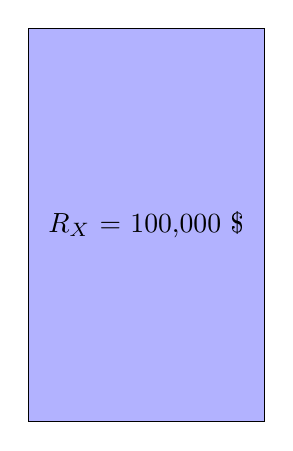
\begin{tikzpicture}
          \node[rectangle,
          fill = blue!30!white,
          minimum width = 3cm,
          minimum height = 5cm,
          draw] (r) at (0,0) { $R_{X}$ = 100,000 \$};
        \end{tikzpicture}
      }
      \only<3>{
        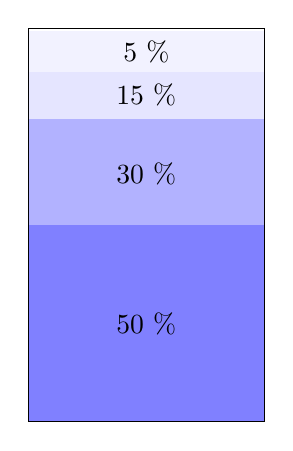
\begin{tikzpicture}
          \node[rectangle,
          fill = blue!5!white,
          minimum width = 3cm,
          minimum height = 0.25cm,
          fill] (r) at (0,2.2) {5 \%};

          \node[rectangle,
          fill = blue!10!white,
          minimum width = 3cm,
          minimum height = 0.6cm,
          fill] (r) at (0,1.65) {15 \%};

          \node[rectangle,
          fill = blue!30!white,
          minimum width = 3cm,
          minimum height = 1.4cm,
          fill] (r) at (0,0.65) {30 \%};

          \node[rectangle,
          fill = blue!50!white,
          minimum width = 3cm,
          minimum height = 2.5cm,
          fill] (r) at (0,-1.25) {50 \%};

          \node[rectangle,
          minimum width = 3cm,
          minimum height = 5cm,
          draw] (r) at (0,0) {};
        \end{tikzpicture}
      }
    \end{column}
    \begin{column}{.5\textwidth}
      \centering\textbf{$Y$ = EUR}

      \only<2>{
        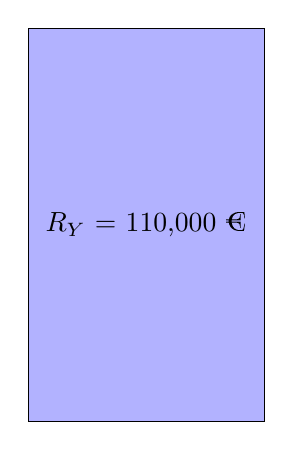
\begin{tikzpicture}
          \node[rectangle,
          fill = blue!30!white,
          minimum width = 3cm,
          minimum height = 5cm,
          draw] (r) at (0,0) { $R_{Y}$ = 110,000 €};
        \end{tikzpicture}
      }
      \only<3>{
        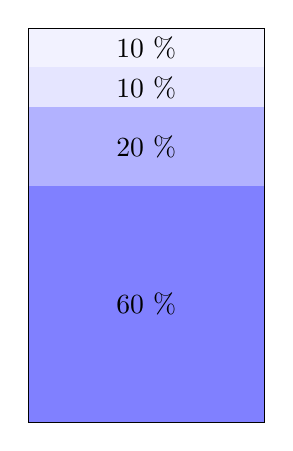
\begin{tikzpicture}
          \node[rectangle,
          fill = blue!5!white,
          minimum width = 3cm,
          minimum height = 0.5cm,
          fill] (r) at (0,2.25) {10 \%};

          \node[rectangle,
          fill = blue!10!white,
          minimum width = 3cm,
          minimum height = 0.5cm,
          fill] (r) at (0,1.75) {10 \%};

          \node[rectangle,
          fill = blue!30!white,
          minimum width = 3cm,
          minimum height = 1cm,
          fill] (r) at (0,1) {20 \%};

          \node[rectangle,
          fill = blue!50!white,
          minimum width = 3cm,
          minimum height = 3cm,
          fill] (r) at (0,-1) {60 \%};

          \node[rectangle,
          minimum width = 3cm,
          minimum height = 5cm,
          draw] (r) at (0,0) {};
        \end{tikzpicture}
      }
    \end{column}
  \end{columns}
  \vspace{2em}
  \centering\only<2>{Звідки вони беруться?}
\end{frame}

\begin{frame}\frametitle{У чому різниця між АММ та біржами на ордер буках?}
  \begin{block}{Чим АММ краща за ордер буки?}
    \begin{itemize}
      \item Прозорість
      \item Детермінованість
      \item Простота в імплементації
    \end{itemize}
  \end{block}

  На цій моделі трейдингу побудовано багато децентралізованих бірж, таких як:

  \begin{itemize}
    \item Uniswap
    \item Curve
    \item SushiSwap
  \end{itemize}
\end{frame}

\end{document}
